\section{Results}
\section{Discretization of PID controller}
The PID-controller was discretized by zero order hold method. The ZOH method give a perfect match between continuous and discrete time domain. This method can also be used for system with input delays, output delays or transport delays and provides an exact discretization. 
The eq. (\ref{eq5}) describes how to transform from s-domain to z-domain using Zero order hold method
\begin{equation} \label{eq5}
    C(z)=(1-z^{-1}) Z(\frac{C(s)}{s}) 
\end{equation}
where C(s) is the controller and Z is the Z-transform
\begin{equation}
    C(z)=(\frac{z-1}{z})Z(\frac{k_Ps+k_I+k_Ds^2}{s} \Big/ s)
    \label{eq7}
\end{equation}
By looking at the z-transform table, the equation \ref{eq7} yields to
\begin{equation}
    C(z)=\frac{z-1}{z}\bigg( k_p \frac{1}{1-z^{-1}}+k_I \frac{T z^{-1}}{(1-z^{-1})^2}+k_D\bigg)
\end{equation}
And finally the PID controller in discrete time domain is presented as
\begin{equation}
    C(z)= k_P + k_I \frac{1}{z-1} + k_D \frac{z-1}{z}
\end{equation}\\

\subsection{Motor simulation}
The PID parameters were chosen to get low settling time, low overshoot and fast response to disturbances for the system. The best parameters for the system resulted in 
\begin{equation}
    \begin{split}
        K_P & = 1.35 \\
        K_I & = 6 \\
        K_D & = 0.08 \\
    \end{split}
\end{equation}
The simulation is made in discrete time domain with a sampling frequency 10 Hz.
\begin{figure}[H]
    \centering
    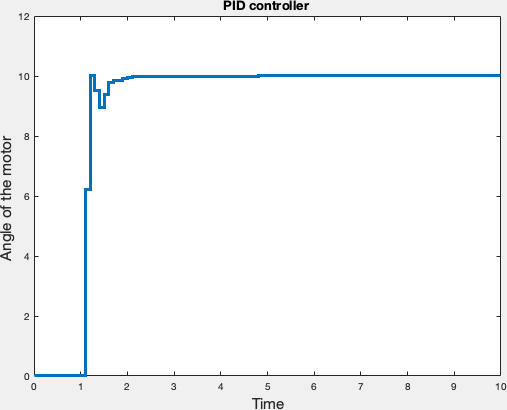
\includegraphics[width=0.4\textwidth]{{sections/assets/pid_motor}
    \caption{PID controller for the LEGO EV3 motor to rotate 10 degrees}
    \label{fig1}
\end{figure}
